%%%%%%%%%%%%%%%%%%%%%%%%%%%%%%%%%%%%%%%%%%
%
% Cosecivi 2017
% http://gaia.fdi.ucm.es/sites/cosecivi17
% 12 pages max
%
%%%%%%%%%%%%%%%%%%%%%%%%%%%%%%%%%%%%%%%%%%

\documentclass{llncs}

\usepackage{float}
\usepackage[english]{babel}
\usepackage[utf8]{inputenc}
\usepackage{epsfig}
\usepackage{graphicx}
\usepackage{subcaption}
\captionsetup{compatibility=false}
\usepackage{color}
\usepackage{amsfonts}
\usepackage{amsmath}
%\usepackage{mathabx}
\usepackage{hyperref}
\hypersetup{
	colorlinks=true,       % false: boxed links; true: colored links
    linkcolor=black,       % color of internal links (change box color with linkbordercolor)
    citecolor=black,        % color of links to bibliography
    filecolor=magenta,      % color of file links
    urlcolor=blue           % color of external links
}
\usepackage{listings}

%\usepackage{hyperref}
%\usepackage{subfigure}
%\usepackage[colorinlistoftodos, textwidth=3.2cm, shadow]{todonotes}

%\usepackage{algorithm}
%\usepackage{fixltx2e}
%\usepackage{algpseudocode}

\usepackage{multirow}

% To use Call inside another Call (algorithms)
%\MakeRobust{\Call}

\graphicspath{{images/}}

\newcommand{\pacman}{Ms. Pac-Man vs. Ghosts }
\newcommand{\paco}{Pac-Man }
\newcommand\tab[1][1cm]{\hspace*{#1}}
\newcommand\menostab[1][-0.5cm]{\hspace*{#1}}

%%%%%%%%%%%%%%%%%%%%%%%%%%%%%%%%%%%%%%%%%%
%
% Title
%
%%%%%%%%%%%%%%%%%%%%%%%%%%%%%%%%%%%%%%%%%%
\title{A Pac-Man bot based on Grammatical Evolution\thanks{Supported by Spanish Ministry of Economy, Industry and Competitiveness under grants TIN2014-55006-R and TIN2014-57028-R}
}

\author{Héctor Laria Mantecón, Jorge Sánchez Cremades, José Miguel Tajuelo Garrigós, Jorge Vieira Luna, Carlos Cervigon Rückauer, Antonio A. S\'{a}nchez-Ruiz}

\institute{
	Dep. Ingenier\'{\i}a del Software e Inteligencia Artificial \\
	Universidad Complutense de Madrid (Spain) \\
	\email{\{hlaria, jorsan06, jtajuelo, jovieira, ccervigon, antsanch\}@ucm.es}
}

\begin{document}

\maketitle
%%%%%%%%%%%%%%%%%%%%%%%%%%%%%%%%%%%%%%%%%%
%
% Abstract
%
%%%%%%%%%%%%%%%%%%%%%%%%%%%%%%%%%%%%%%%%%%
\begin{abstract}
In this article, we propose the development of a bot for playing the video game \pacman using a grammatical evolution based evolutionary algorithm. This technique evolves programs that are evaluated by executing them in the game. The program encodes the strategy that the bot plays and is obtained through the derivation of grammar rules in a particular order, which is defined by the algorithm.
We experimented with two different grammars: The first one includes high-level actions and the second one involves medium-level actions. Both grammars include state providers. To make the evolutionary process more efficient, we perform a series of optimizations on the evolutionary algorithm, including parallelization of the fitness evaluation and multi-objective optimization.
Experimental results using the two grammars and two different ghost controllers  are presented. We report better results with our bots than the baseline controllers and other controllers based on grammatical evolution.

% orientarlo a que no funciona el multi (depsues) //// (ya esta puesto al final que  se exploraran los resultados del multi, le veo mas sentido a eso que a poner aqui si funciona mejor o peor)

% In this work we study Ms. Pac-Man vs Ghosts bot development using gramatical evolution. We make use of derivation trees to represent programs that Pac-Man runs to play. The programs are evolved using a grammatical evolution algorithm.
% When a program is produced from its grammar, we parse the code and generate a game tree. For the Pac-Man controller to query a movement from that tree every turn, all it has to do is navigate the tree from the root down to a terminal node.

% We will be using "medium level" and "high level" grammars, the former using calls to a set of functions that extract raw information from the game, the latter using more complex functions created by us that mix raw information with expert-knowledge. 

% To make the evolution process more efficient, we perform a series of optimizations to the evolutionary algorithm. These include running parallel evaluations to save time, and creating multi-objective fitness functions to better guide the evolution process. We will be exploring the results of multi-objective optimization in detail.

\end{abstract}

\keywords{Genetic programming, grammatical evolution, multi-objective optimization, decision trees, Pac-Man}
%reactive artificial intelligence, bots in video-games}

%%%%%%%%%%%%%%%%%%%%%%%%%%%%%%%%%%%%%%%%%%
%
\section{Introduction}
\label{sec:intro}
%
%%%%%%%%%%%%%%%%%%%%%%%%%%%%%%%%%%%%%%%%%%


% lo único que podría contarse mas es que es GE o PG, pero eso va en el punto dos, sería redundante
Ever since the birth of video-games we’ve seen artificial intelligence techniques applied to them: Character behaviour, enemy strategies, path-finding, etc. We want to explore Grammatical Evolution (a Genetic Programming variant) to evolve game strategies generated from the derivation of defined grammar rules. For this purpose, we experimented with the evolution of a bot for Ms. Pac-Man, a well-known game which can have many sub-goals, like surviving the most time possible, eating the most pills, killing as many ghosts as it can, or go through a lot of levels before dying to the ghosts.

Particularly, we experimented with controllers based on two different grammars, with high and medium level actions respectively. Due to the complexity of video-games and how useful it could be for an artificial intelligence to modify its behaviour in real time, we want to check the results of multi-objective optimization in grammatical evolution, and how we can achieve the sub-goals we consider more important in a situation by simply changing the evaluation functions we use in the grammatical evolution algorithm.

We will show that this approach based on Grammatical Evolution gets excellent results and we will see that the bots produced can obtain high scores and complete several levels, even better results than the coded bots included, or other known evolutionary bots.

The rest of the article is structured as follows: Section 1 describes the techniques and the work we’ve found related to our project. Section 3 gives information on the \paco framework we use and the bots we experiment with. Section 4 explain our bot in detail showing some results and comparatives. Section 5 describes multi-objective optimization and its results, and we will compare them to the previous ones. Finally, in section 6, we discuss the conclusions of this study and the future work.


%The rest of the paper is organized as follows. Section~\ref{sec:tetris-analytics} describes the specific version of Tetris used in our experiments. Section~\ref{sec:player-modeling} explains our CBR approach to model and dynamically detect the skill level of the player. Next, Section~\ref{sec:dda} describes how we change the difficulty of the game dynamically according to the player profile. Section \ref{sec:experiments-results} explains the experiment performed with real players and the different effects observed with and without DDA. Finally, the paper closes with related work, conclusions and future work.    


%%%%%%%%%%%%%%%%%%%%%%%%%%%%%%%%%%%%%%%%%%
%
\section{Related Work}
\label{sec:relatedWork}
%
%%%%%%%%%%%%%%%%%%%%%%%%%%%%%%%%%%%%%%%%%%

\subsection{Genetic Programming}

Genetic Programming (GP)~\cite{poli_langdon_mcphee_koza_2008} is one of the many different branches of algorithms that exist in the field of Evolutionary Algorithms. The goal in GP is to produce the best program, in a determined programming language, to solve a particular program. The programs are usually encoded using a tree structure (genotype) in which each node represents a token of the chosen programming language. Certain individuals in the population will be selected, recombined and transformed slightly by different types of selection, crossover and mutation operators.
In order to evaluate the performance of each individual, its genome will be transformed into the final program (phenotype) that will be executed in the context of the particular problem to solve. This process is repeated several times and the final solution will be the individual representing the program with the best score of the whole population~\cite{cervigon}. 

The main drawback of GP is that the use of trees to encode the genotype is very demanding in terms of memory, especially when bloating occurs~\cite{Poli2003}, and that the selection, crossover and mutation operators are relatively slow because they work with recursive tree structures.

GP has been used previously to evolve AI controllers for the Pac-Man game. In particular, Koza~ \cite{koza1992genetic} used a set of high level operators for maze information retrieval (\textit{DISF - Distance to Fruit}) and Pac-Man direct control (\textit{AFRUIT - Advance to Fruit}) to develop a bot for a custom version of the game. Alhejali and Lucas~\cite{alhejali_lucas_2010} also used GP with even more abstract operators (\textit{isInDanger(takes two arguments), IsToEnergizerSafe(takes two arguments) or toSafety}) to automatically evolve Pac-Man players. Brandstetter and Ahmadi~\cite{brandstetter_ahmadi_2012}, on the other hand, used low level action operators for Pac-Man movement (\textit{UP, DOWN...}), obtaining better results (score) compared with the previous controllers.

\subsection{Grammatical Evolution}

Grammatical Evolution (GE)~\cite{o'neill_ryan_2012} is similar to Genetic Programming in that both evolve programs to find the best one to solve a particular problem, but they differ on the encoding (genotype). While GP uses trees, GE uses an array of integers where each integer represents the rule of the grammar (in BNF) that will be chosen to produce the program (phenotype) when the genotype is decoded. That is, instead of storing the syntactic tree, in GE each individual stores information to derive the program from the language grammar. This way, the process of crossover and mutation works with integer arrays, it is much faster and consumes less memory. The algorithm is also independent from the domain, so we can solve different problems just changing the grammar to define the space of valid programs. 

Although classical crossover operators, like the single-point crossover, and classical mutation operators, like integer flip mutation, can be used in GE algorithms, they tend to produce too much noise in the phenotype, especially crossover which generates chaotic populations. For this reason, new operators had been developed to try to avoid this destructive behaviour, like LHS replacement crossover, which tries to do the crossover less destructive by taking into account the phenotype structure and not just the genotype~\cite{harper_blair_2005} and Neutral Mutation for improving population's diversity~\cite{oesch_maringer_2014}.

Grammatical Evolution (GE) has also been previously used to evolve Pac-Man controllers. Galván-López~\cite{galvan2010evolving} used a similar approach to Koza's using high level operators for movement (\textit{ANG - Avoid Nearest Ghost}) and information retrieval (\textit{avgDistBetGhosts}). They used a grammar with if-else statements to achieve determined outputs based on some game conditions. With this approach, they achieved similar results to GP controllers with the advantage that the BNF could be changed easily changing adding restrictions or features easily. 

Liberatore~\cite{Liberatore2014} proposed another interesting approach using GE and Flocking Strategies to develop a Swarm-type intelligent for the Pac-Man ghost's controllers. 

%%%%%%%%%%%%%%%%%%%%%%%%%%%%%%%%%%%%%%%%%%
%
\section{\pacman}
\label{sec:pacmanai}
%
%%%%%%%%%%%%%%%%%%%%%%%%%%%%%%%%%%%%%%%%%%

\begin{figure}[tb]
	\centering
	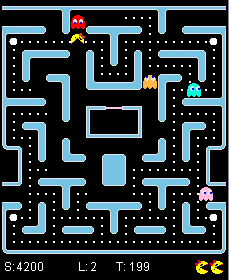
\includegraphics[width=0.50\textwidth]{images/PacMan_ss.png}
	\caption{\pacman videogame.}
	\label{fig:pac-man}
\end{figure}

\pacman (Figure~\ref{fig:pac-man}) is a very popular arcade video game. In the version that we use~\cite{mspacmangithub}, there is a set of four pre-generated toroidal 2D labyrinths, in which the ghosts and \paco move. The ghosts always start in the ``Lair'', a rectangle in the middle of the map in which \paco cannot enter, while \paco starts in the bottom of the map. 

Each labyrinth is composed of corridors and junctions filled with a lot of pills and four power pills. Both give points to \paco as he walks over them, and power pills make him able to eat the ghosts for a short period of time, while also slowing them. Eating ghosts will give \paco points, earning some extra ones if he eats various ghosts in a row during the same power pill buff duration.

\paco will try to eat all the pills and power pills to advance levels, while avoiding the ghosts, which will try to hunt him, making him lose a live when they walk over him. A level is completed when there are no pills and power pills left, and there are an infinite number of levels, repeating the same set of 4 labyrinths consecutively.

\paco will strive to eat all the pills and power pills in the map to advance levels, while trying to get as many points as possible (eating any ghosts he can), since each 10.000 points achieved he gets an extra life. The game ends either when \paco loses his three lives or after 24.000 turns, considering a turn passes every time both \paco and the ghosts make a movement.

\pacman has been used in different competitions in which participants have used several different AI techniques in order to create the best automatic player. The most important competitions are \emph{cha. Pac-Man Competition}~\cite{mspacmancompetitionwebsite} and \emph{Ms. Pac-Man Vs. Ghost Team Competition}~\cite{pacmanvsghostsaiwebsite} \cite{pmvsghostspaper2016}

\subsection{Bot implementation architecture}

Both the ghosts and \paco use controllers to determine which movement is the best to make every turn. These controllers are the ones that must be implemented to participate in the competitions, which can be done using any technique available.

Every turn the game provides the controllers with its current state, so that the controller can seek relevant information it needs to choose a movement. Such information includes the pre-calculated distance from a point of the map to another (useful to check distances between \paco and the ghosts), which is the movement that puts you further away from any other position (useful to run away from the ghosts), which movements are possible given a position, testing if a position is a junction or not, etc. 

%We've greatly increased the information to obtain by combining those given functions, like getting a movement towards the closest junction, the closest edible ghost, or the closest power pill.

The original code also provides various examples of controllers like random movements for \paco and the ghosts, aggressive behavioural ghosts, or a basic one for \paco that considers if the surrounding ghosts are edible or not. In particular, we use 2 different ghost's controllers in our experiments:

\begin{itemize}
\item \emph{Random}: ghosts make random decisions.
\item \emph{Legacy}: it tries to reproduce the behaviour in the original game where each ghost used different heuristics to move.
\end{itemize}


%%%%%%%%%%%%%%%%%%%%%%%%%%%%%%%%%%%%%%%%%%
%
\section{A bot based on grammatical evolution}
\label{sec:sec1}
%
%%%%%%%%%%%%%%%%%%%%%%%%%%%%%%%%%%%%%%%%%%

We use Grammatical Evolution (GE) to evolve \paco controllers which play the game automatically. The type of programs that we consider valid \paco controllers are defined using a context-free grammar. This way, we can reduce and refine the search space the evolutionary algorithm will explore, and focus on certain type of programs that we think more promising. In particular, we are going to evolve decision trees in which the internal nodes check game conditions and the leaves describe specific actions to execute in the game.

\begin{figure}[tb]
	\centering
% \begin{lstlisting}[frame=single, breaklines=no, basicstyle=\fontsize{10}{11}\ttfamily]
%         if (dist_closest_NE_ghost < 10) {
%             escape
%         } else {
%             seekFood
%         }
% \end{lstlisting} % con o sin frame
\begin{lstlisting}[frame=single, breaklines=no, basicstyle=\fontsize{10}{11}\ttfamily]
        if (dist_closest_NE_ghost < 10) { escape } 
        else { seekFood }
\end{lstlisting} % con o sin frame
	\caption{Example of a simple controller based on a decision tree.}
	\label{fig:example}
\end{figure}

For example, the program in Figure~\ref{fig:example} describes a very simple bot that runs when there is a ghost near, and moves towards the closest pill in other case. 

In the general case, conditional statements can have other conditional statements inside and, therefore, the bot can take decisions based on more complex analysis of the game state. Note that, although decisions trees only allow to define reactive bots (we cannot encode explicitly advanced strategies consisting of action sequences), the evaluation of these decision trees at every game turn can produce very complex behaviours. 

In order to implement a \paco bot based on GE, we use the JECO (\textit{Java Evolutionary COmputation library})~\cite{jecorepo} framework which supports different evolutionary computation techniques, including simple and multi-objective grammatical evolution.

\subsection{Grammar design}

We use 2 different types of terminals in our grammars:

\begin{itemize}
\item \textbf{Actions}. They represent Java methods that return a concrete move for the bot to execute. This way, we can use both abstract behaviours like \emph{escape} or concrete moves like \emph{left}.

\item \textbf{State providers}. They represent Java methods that return information of the current game state either as boolean or numeric values. For example, \emph{dist\_closest\_NE\_ghost} returns the distance to the closest non-edible ghost.
\end{itemize}

We decided to design two grammars. The first one includes high level actions (strategies coded in Java) and state providers, while the second one includes medium-level actions and state providers. Both grammars contain conditional statements (if / if-else), numeric constants and numeric operators (\texttt{==, !=, >, >=, <, <=}). Our goal is to work at different levels of abstraction and study the effect in both the search space and the optimality of the resulting program. 

\begin{figure}[tb]
	\centering
\begin{lstlisting}[frame=single, breaklines=false, basicstyle=\fontsize{10}{11}\ttfamily]
<grammar>  ::= <sel-stat>
<sel-stat> ::= if(_<cond>_){_<stat>_}_else{_<stat>_}
               | if(_<cond>_){_<stat>_}
<stat>     ::= <action> | <sel-stat>
<action>   ::= escape | attack | seekFood
<cond>     ::= <num-st>_<num-op>_<num>
<num-st>   ::= dist_closest_NE_ghost
              | dist_closest_E_ghost
<num-op>   ::= EQ | NE | LT | GT | LE | GE
<numb>     ::= 0 | 5 | 10 | ... | 40
\end{lstlisting} % con o sin frame
	\caption{High-level grammar.}
	\label{fig:hl-grammar}
\end{figure}

Figure \ref{fig:hl-grammar} shows the high-level grammar that contains 3 high-level actions: \emph{escape} (run from the closest ghost), \emph{attack} (go to the closest ghost) and \emph{seekFood} (go to the closest pill). It only contains 2 state providers: distances to the closest edible and non-edible ghost.

\begin{figure}[tb]
	\centering
\begin{lstlisting}[frame=single, breaklines=false, basicstyle=\fontsize{10}{11}\ttfamily]
<gram>     ::= <sel-stat>
<sel-stat> ::= if(_<cond>_){_<stat>_}_else{_<stat>_}
               | if(_<cond>_){_<stat>_}
<stat>     ::= <action> | <sel-stat>
<action>   ::= run_to_closest_pill 
               | run_to_closest_ppill 
               | run_to_closest_E_ghost 
               | run_from_closest_NE_ghost
<cond>     ::= <bool-st>  
               | <num-st>_<num-op>_<num> 
<bool-st>  ::= <bool-api> | not _<bool-api>
<bool-api> ::= is_junction
<num-st>   ::= dist_closest_NE_ghost
               | dist_closest_NE_ghost 
               | dist_closest_pill
               | ...
<num-op>   ::= EQ | NE | LT | GT | LE | GE
<numb>     ::= 0 | 5 | 10 | ... | 40
\end{lstlisting} % con o sin frame
	\caption{Medium-level grammar.}
	\label{fig:ml-grammar}
\end{figure}

Figure \ref{fig:ml-grammar} shows the medium-level grammar that contains 4 actions to run to the closest pill, power pill, edible ghost and run away form the closest non-edible ghost. This grammar has several more state providers in order to create more complex conditions.

\textbf{Medium-level state providers:}
\textit{Distance to the closest non-edible ghost, distance to the closest edible ghost, number of active power pills, distance to the closest pill, distance to the closest power pill, geometric mean of the distances to all non-edible ghost, geometric mean of the distances to all edible ghost}

\textbf{Medium-level actions:}
\textit{Run to closest pill, run to closest power pill, run away from closest non-edible ghost, run to closest edible ghost}

\textbf{High-level actions:}
\textit{escape, attack, seekFood}
\begin{itemize}
\addtolength{\itemindent}{1cm}
\item \textit{escape}: \paco moves towards the closest pill if he can reach it before any ghost, or runs away from the closest ghost if he can't (Also runs away if there are no power pills left).
\item \textit{attack}: \paco moves towards the closest edible ghost if no other ghost can reach the edible one before him. If there are no edible ghosts, \paco moves in the same direction as he did in the previous turn.
\item \textit{seekFood}: \paco moves towards the closest pill if he can reach it before any ghost does. If there are no more pills, moves towards the closest power pill.
\end{itemize}

%<number-func> ::= getDistanceToClosestNonEdibleGhost
%                | getDistanceToClosestNonEdibleGhostUp
%                | getDistanceToClosestNonEdibleGhostDown
%                | getDistanceToClosestNonEdibleGhostLeft
%                | getDistanceToClosestNonEdibleGhostRight
%                | getDistanceToClosestEdibleGhost
%                | getDistanceToClosestEdibleGhostUp
%                | getDistanceToClosestEdibleGhostDown
%                | getDistanceToClosestEdibleGhostLeft
%                | getDistanceToClosestEdibleGhostRight
%                | getNumberOfActivePowerPills
%                | getDistToClosestPillUp
%                | getDistToClosestPillDown
%                | getDistToClosestPillLeft
%                | getDistToClosestPillRight
%                | getDistToClosestPill
%                | getDistToClosestPowerPill
%                | getDistToClosestPowerPillUp
%                | getDistToClosestPowerPillDown
%                | getDistToClosestPowerPillLeft
%                | getDistToClosestPowerPillRight
%                | getClosestJunctionExitsNumberUp
%                | getClosestJunctionExitsNumberDown
%                | getClosestJunctionExitsNumberLeft
%                | getClosestJunctionExitsNumberRight
%                | getDistanceToClosestJunctionUp
%                | getDistanceToClosestJunctionDown
%                | getDistanceToClosestJunctionLeft
%                | getDistanceToClosestJunctionRight
%                | getClosestNonEdibleGhostDistanceToClosestJunctionUp
%                | getClosestNonEdibleGhostDistanceToClosestJunctionDown
%                | getClosestNonEdibleGhostDistanceToClosestJunctionLeft
%                | getClosestNonEdibleGhostDistanceToClosestJunctionRight
%                | getClosestEdibleGhostDistanceToClosestJunctionUp
%                | getClosestEdibleGhostDistanceToClosestJunctionDown
%                | getClosestEdibleGhostDistanceToClosestJunctionLeft
%                | getClosestEdibleGhostDistanceToClosestJunctionRight
%                | getGeometricMeanDistanceToNonEdibleGhosts
%                | getGeometricMeanDistanceToEdibleGhosts


\subsection{Operators and Fitness function}

After several tests comparing selection, elite, crossover and mutation operators as well as their hyper-parameters, we obtained the best results using: Binary Tournament selection\cite{binarytour} with 5\% elite, LHS crossover~\cite{harper_blair_2005} with 60\% probability and Integer Flip mutation with 10\% probability and using Neutral mutation~\cite{oesch_maringer_2014}.

To maximize the score of the controller we minimize the following fitness function:
\begin{equation*} % label: naivefitness
f = 100000 - score
% caption: Naive fitness
\end{equation*}

\paco obtains points every time he eats a pill (10 points), a power pill (50 points) or an edible ghost (200 points). When \paco eats more than one ghost in a row, he gets extra points (400 for the second ghost, 800 for the third, ...).

\subsection{Results}

We performed 4 experiments evolving bots with the previous 2 grammars and using 2 different ghost controllers: Random and legacy. Note that the legacy ghosts are much more challenging than the random ghosts. We also compared our bots with the UCD Dublin bot~\cite{galvan2010evolving}, another bot trained using Grammatical Evolution and high-level actions and state providers.

All the experiments were run using the same configuration: Population size 100, Generations 100, 30 games played per individual evaluation, Binary Tournament selection, LSH crossover (60\%), Integer Flip mutation (10\%), Neutral mutation and elitism (5\%).


\begin{figure}[tb]
   \centering
    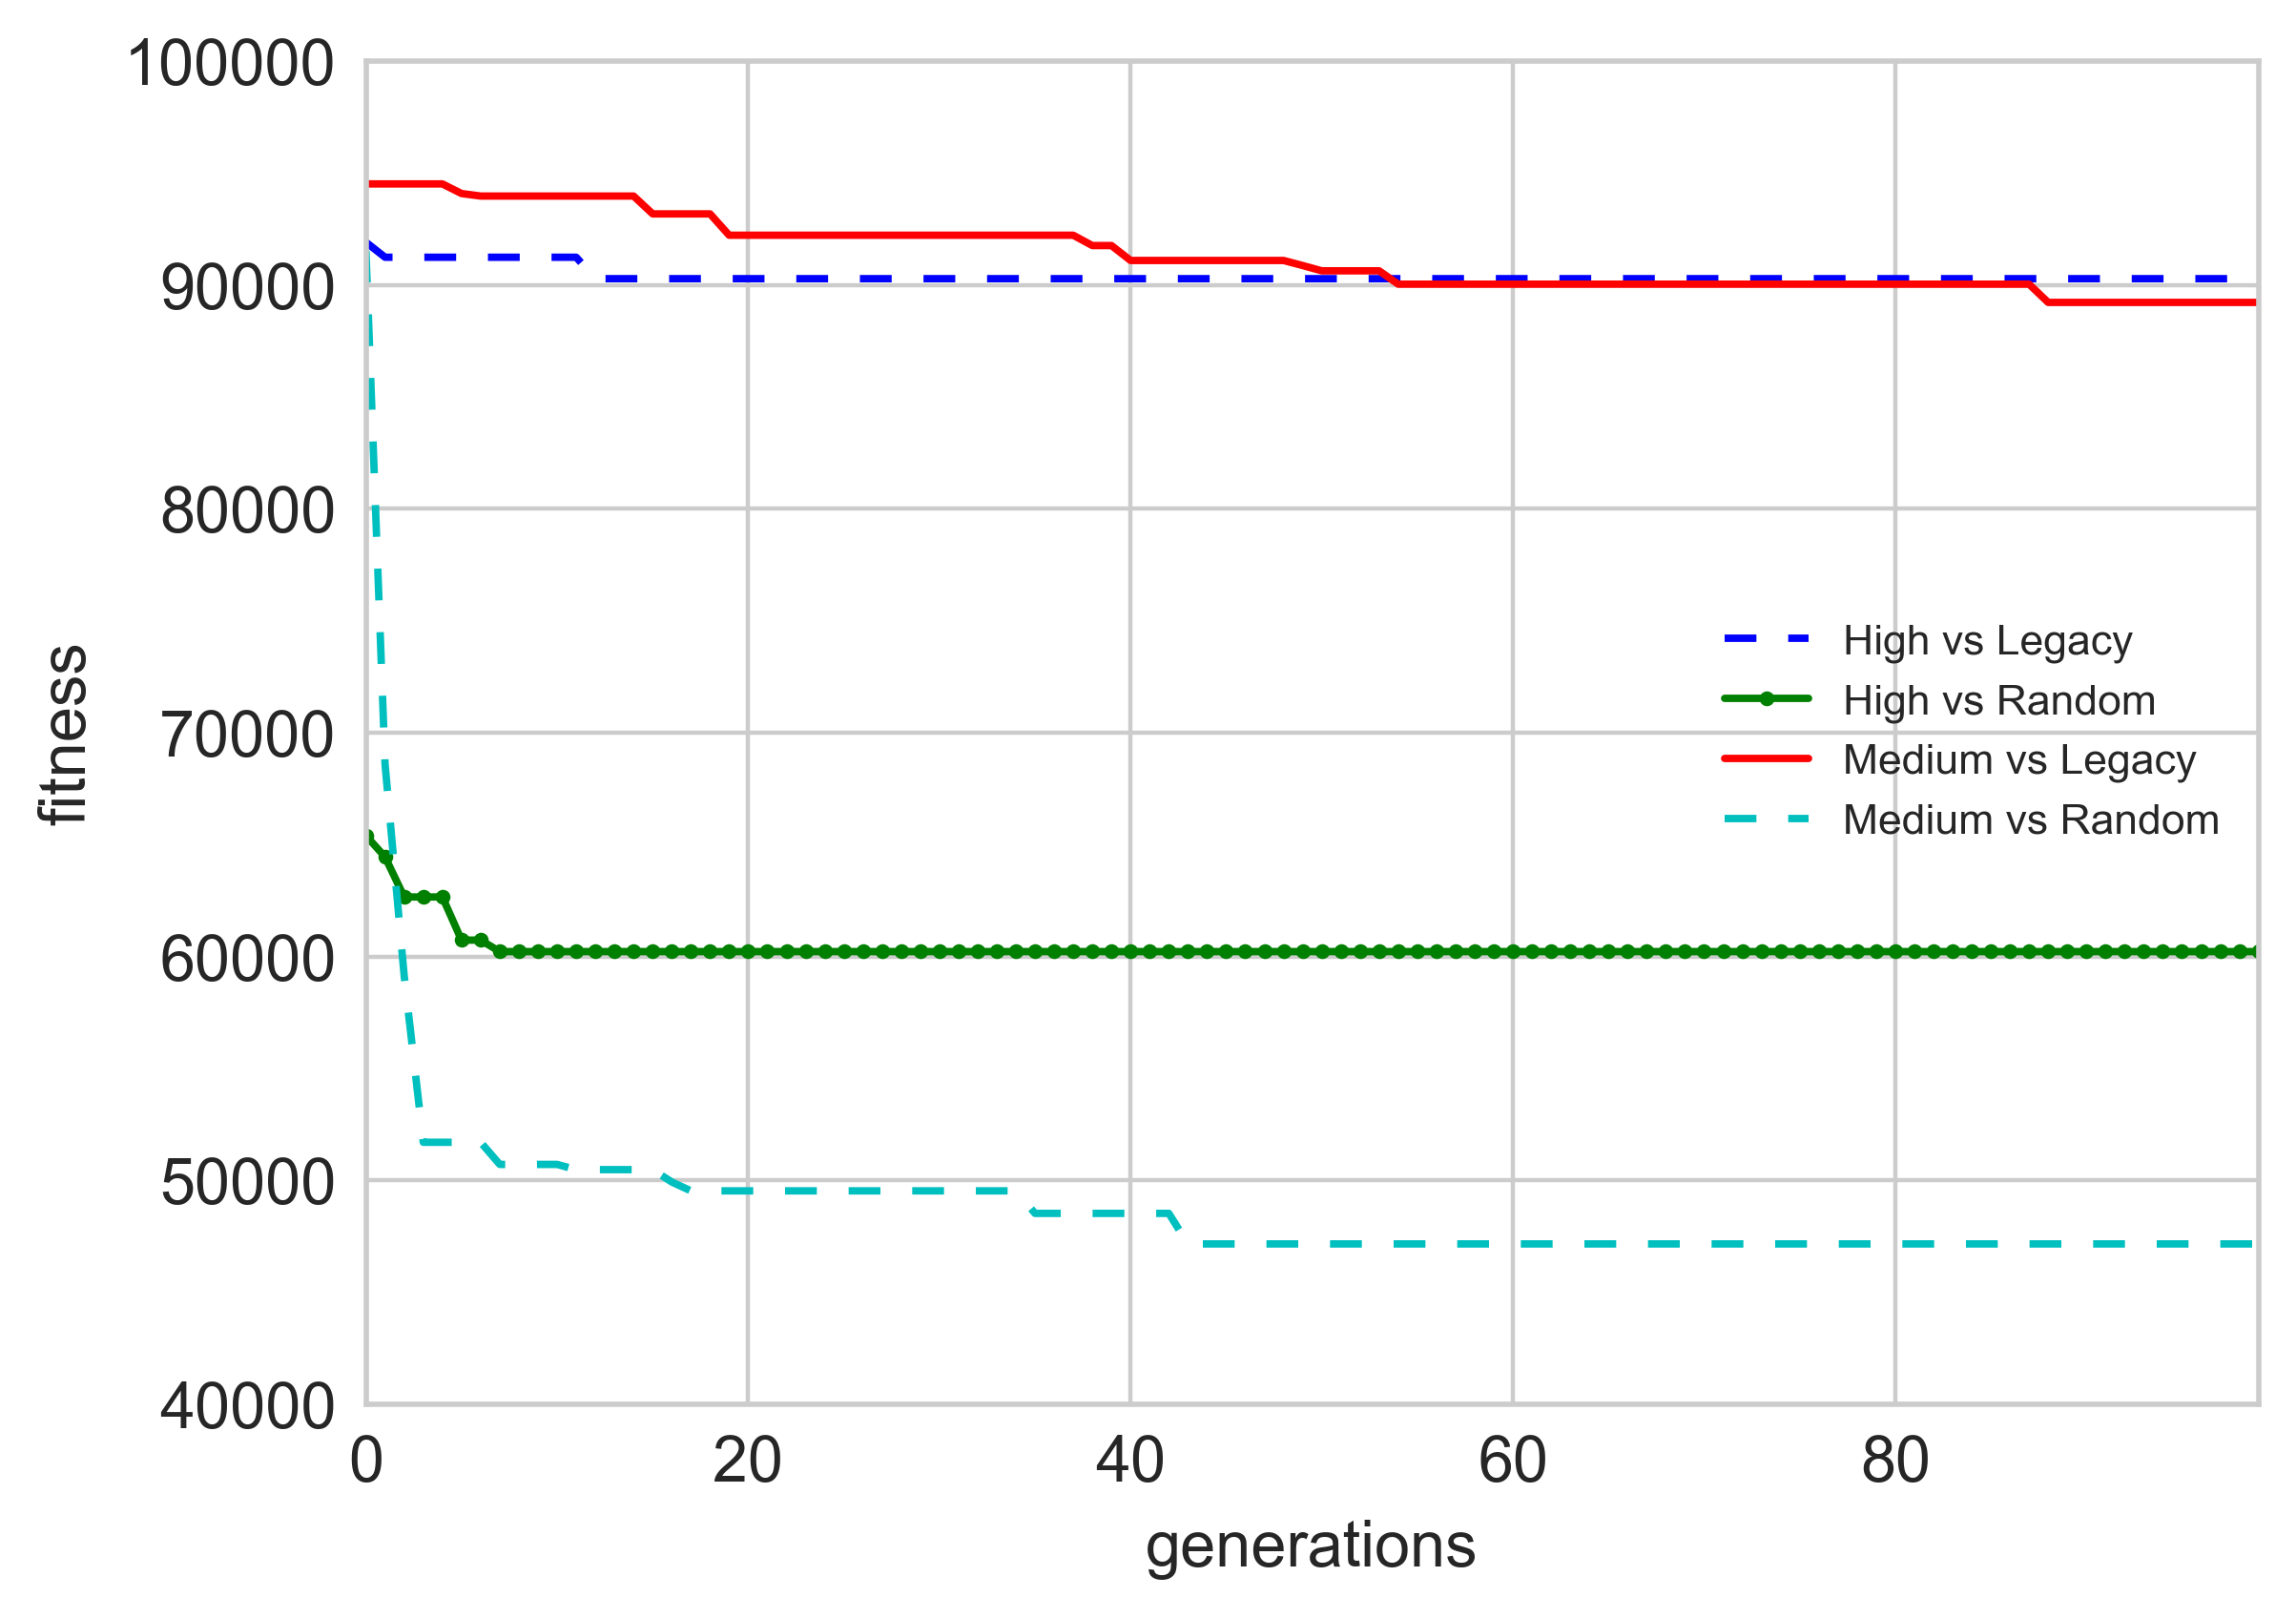
\includegraphics[width=0.9\textwidth]{so_fitness_bests}
    \caption{Fitness evolution vs. generation (less is better).}
    \label{fig:fitness}
\end{figure}

Figure \ref{fig:fitness} shows the evolution of the fitness function as we produce new generations of individuals in each experiment.

\begin{table}[]
\centering
\caption{\paco vs Ghost controllers' comparison.}
\label{table:single_obj}
\begin{tabular}{|l|c|r|r|r|r|r|r|r|r|r|}
\hline
\multicolumn{1}{|c|}{\multirow{2}{*}{\textbf{\paco}}} & \multirow{2}{*}{\textbf{Ghosts}} & \multicolumn{3}{c|}{\textbf{score}} & \multicolumn{3}{c|}{\textbf{level}} & \multicolumn{3}{c|}{\textbf{time (game ticks)}} \\ \cline{3-11} 
\multicolumn{1}{|c|}{} &  & \multicolumn{1}{c|}{\textbf{max}} & \multicolumn{1}{c|}{\textbf{avg}} & \multicolumn{1}{c|}{\textbf{std}} & \multicolumn{1}{c|}{\textbf{max}} & \multicolumn{1}{c|}{\textbf{avg}} & \multicolumn{1}{c|}{\textbf{std}} & \multicolumn{1}{c|}{\textbf{max}} & \multicolumn{1}{c|}{\textbf{avg}} & \multicolumn{1}{c|}{\textbf{std}} \\ \hline
Random &  \multirow{5}{*}{Random} & 1380 & 501 & 213 & 1 & 0.036 & 0.186 & 5635 & 1943 & 887.5 \\ \cline{1-1} \cline{3-11} 
NearestPill &  & 18910 & 4471 & 2654 & 5 & 1 & 0.9 & 7216 & 1795 & 1018 \\ \cline{1-1} \cline{3-11} 
UCD Dublin bot\cite{galvan2010evolving} &  & 11640 & 4288 & - & - & - & - & - & - & - \\ \cline{1-1} \cline{3-11} 
\textbf{Medium-level} &  & \textbf{64600} & \textbf{48558} & \textbf{10780} & \textbf{18} & \textbf{15} & \textbf{3.4} & \textbf{24000} & \textbf{21579} & \textbf{4470} \\ \cline{1-1} \cline{3-11} 
\textbf{High-level} &  & \textbf{55480} & \textbf{32704} & \textbf{13237} & \textbf{18} & \textbf{10.4} & \textbf{4.3} & \textbf{24000} & \textbf{17457} & \textbf{6784} \\ \hline
Random & \multirow{5}{*}{Legacy} & 1840 & 197 & 107 & 0 & 0 & 0 & 877 & 465 & 61.3 \\ \cline{1-1} \cline{3-11} 
NearestPill &  & 7190 & 3531 & 638 & 1 & 0.4 & 0.5 & 1881 & 1152 & 143.7 \\ \cline{1-1} \cline{3-11} 
UCD Dublin bot\cite{galvan2010evolving} &  & 12350 & 3945 & - & - & - & - & - & - & - \\ \cline{1-1} \cline{3-11} 
\textbf{Medium-level} &  & \textbf{15960} & \textbf{6358} & \textbf{2883} & \textbf{3} & \textbf{0.9} & \textbf{0.7} & \textbf{4973} & \textbf{1916} & \textbf{730} \\ \cline{1-1} \cline{3-11} 
\textbf{High-level} &  & \textbf{20040} & \textbf{5972} & \textbf{2832} & \textbf{4} & \textbf{1} & \textbf{0.6} & \textbf{8364} & \textbf{2026} & \textbf{1020} \\ \hline
\end{tabular}
\end{table}

Table~\ref{table:single_obj} displays the results of the experiments. In each experiment we measure the final score, the level reached and the time played showing the maximum, average and standard deviation values of 1000 games. As we were expecting, the \emph{Legacy} ghosts are more challenging opponents than the \emph{Random} ghosts and all the values are smaller because the games are much shorter. 

Both our grammars can produce bots that play better than the baseline controllers (a random controller and other one that always goes towards the closest pill). Besides, our bots play better than the UCD Dublin bot, and that is interesting because all of them are created using Grammatical Evolution. This seems to happen due to the usage of excessively specific functions which limit its behaviour, i.e. forcing \paco to wait next to a power pill. Their bot also uses large amount of parameters like dimensions of a frame (centered on Pac-Man) to evaluate certain conditions. Conversely, we make use of path distances and numeric operators, resulting in a less complex game status analysis.

Using the medium-level grammar we obtain better results than using the high-level grammar in average, probably because the actions and state providers make possible to create controllers that exploit scenarios that cannot be exploited using the high-level grammar. However, the high-level grammar obtains better results in some particularly good games (max. values). The best evolved controller using the medium-level grammar playing against the Legacy ghosts is able to obtain 6358 points and complete almost 1 level in average. In the best games, this same controller is able to obtain 15960 points and complete 3 levels.

When we analysed the behaviour of the evolved controllers we discovered interesting facts. The bots generated by the high-level grammar share almost always the same code, and achieve slightly lower scores, eating pills conservatively by avoiding ghosts. However, the medium-level grammar tends to generate bots which manage to get stuck next to power pills (stopping themselves), wait for the ghosts to be close and proceeding to eat first the power pill and then the ghosts, now edible. This hunter behaviour allows \paco bots to achieve notable scores, because there is a multiplicative bonus when \paco eats several ghosts in a row.

We also made experiments playing against the \emph{Starter} ghosts controller, a basic implementation that run away when the ghosts are edible and chase \paco with certain probability when they are not edible. Most of the executions using the medium-level grammar evolved controllers able to exploit a bug in the code. They went in circles forever in a corner of the board completing levels (a level can be completed just waiting enough turns) and not being chased by the ghosts.

\begin{figure}[tb]
	\centering
% \begin{lstlisting}[frame=single, breaklines=false, basicstyle=\fontsize{10}{11}\ttfamily]
% if(dist_closest_NE_ghost > 10) {
%     if(dist_closest_NE_ghost < 20) {
%         run_to_closest_ppill 
%     } 
%     else {
%         run_to_closest_pill
%     }
% }
% else {
%     run_from_closest_NE_ghost
% }
% \end{lstlisting} % con o sin frame
\begin{lstlisting}[frame=single, breaklines=false, basicstyle=\fontsize{10}{11}\ttfamily]
if (dist_closest_NE_ghost > 10) {
    if (dist_closest_NE_ghost < 20) { 
    	run_to_closest_ppill 
    } else { run_to_closest_pill }
} else { run_from_closest_NE_ghost }
\end{lstlisting} % con o sin frame
	\caption{Example of controller evolved using the medium-level grammar against the random ghosts.}
	\label{fig:program}
\end{figure}

Regarding the type of generated programs, Figure~\ref{fig:program} shows an example of controller evolved using the medium-level grammar against the random ghosts. Basically, \paco runs away from non-edible ghosts when they are very close, goes towards the closest power pill when the ghosts are close (but not very close), and eats pills in other case.

%\subsubsection{Medium-Level evolved against Random Ghost program} Using Population size 100, Generations 80, 30 games played per individual, Binary Tournament selection, LSH crossover (60\%), Integer Flip mutation (10\%), Neutral mutation and elitism (5\%)
%
%%si lo quieres coger de un archivo usa \lstinputlisting[language=Python]{source_filename.py}

%
%\subsubsection{Medium-Level evolved against Legacy Ghost program} Using Population size 180, Generations 100, 30 games played per individual, Binary Tournament selection, LSH crossover (60\%), Integer Flip mutation (10\%), Neutral mutation and elitism (5\%)
%
%%si lo quieres coger de un archivo usa \lstinputlisting[language=Python]{source_filename.py}
%\begin{lstlisting}[frame=single, caption=Medium-Level evolved against Legacy Ghost]
%if(distClosNEGhost >= 20) {
%    toClosP
%}
%else {
%    if(distClosNEGhostUp != 15) {
%        toClosPP
%    }
%    else {
%        toClosP
%    }
%}
%\end{lstlisting} % con o sin frame
%
%\subsubsection{High-Level evolved against Random or Legacy Ghosts program} Using Population size 100, Generations 50, 30 games played per individual, Binary Tournament selection, LSH crossover (60\%), Integer Flip mutation (10\%), Neutral mutation and elitism (5\%)
%
%%si lo quieres coger de un archivo usa \lstinputlisting[language=Python]{source_filename.py}
%\begin{lstlisting}[frame=single, caption=High-Level evolved against Random or Legacy Ghosts]
%if(distClosNEGhost > 5) {
%    seekFook
%}
%else {
%    escape
%}
%\end{lstlisting} % con o sin frame


%%%%%%%%%%%%%%%%%%%%%%%%%%%%%%%%%%%%%%%%%%
%
\section{Multi-objective optimization}
\label{sec:sec3}
%
%%%%%%%%%%%%%%%%%%%%%%%%%%%%%%%%%%%%%%%%%%

Multi-objective optimization arises when a single objective may not adequately represent the problem being faced, so modelling it with several objectives is preferred. In multi-objective optimization, there are therefore $n$ different objectives each one with its own fitness function $f_i$:
\begin{equation*}
\begin{aligned}
f_i(X) | i = 1,...,n
\end{aligned}
\end{equation*}

The difficulty of this kind of problems lies on determining which individual optimizes all the objectives better. We say that a solution is a Pareto optimal if none of the objective functions can be improved in value without degrading some of the other objective values~\cite{cervigon}. 

Exist a wide variety of methods when implementing a multi-objective algorithm. The easiest consists in creating a fitness function which is a linear combination of all other functions to optimize. The main problem concerns the difficulty to find the adequate weights.

Another popular approach that we will use in this work is the \textit{NSGA-II}~\cite{nsgapaper} algorithm, which delivers very good results yet is computationally expensive, especially for large populations.

\subsection{Why to apply it}

Using a single objective function that maximizes score, inevitably leads to bots that keep moving around a power pill until one or more ghosts approach, at which point \paco eats the power pill and proceeds to eat as many ghost as possible, exploiting the ghost score multiplier.

This strategy only works when there are still power pills available. With no power pills left \paco keeps rambling until a ghost eats it and the game is over. The consequence is that the controller usually is not able to complete more than one level. In order to complete more, we tried to model a multi-objective problem with 2 different fitness functions:
\begin{eqnarray*}
f_2 & = & 100 - \text{last level reached}\\
f_3 & = & 100000 - \text{score}
\end{eqnarray*}

With this functions we create a set $F = [f_2, f_3]$ that will be used by NSGA-II to evolve the population.

\subsection{Results}

\begin{table}[tb]
\centering
\caption{\paco vs Ghost controllers' comparison including Multi-Objective}
\label{table:multi-objective}
\begin{tabular}{|l|c|r|r|r|r|r|r|r|r|r|}
\hline
\multicolumn{1}{|c|}{\multirow{2}{*}{\textbf{\paco}}} & \multirow{2}{*}{\textbf{Ghosts}} & \multicolumn{3}{c|}{\textbf{score}} & \multicolumn{3}{c|}{\textbf{level}} & \multicolumn{3}{c|}{\textbf{time (game ticks)}} \\ \cline{3-11} 
\multicolumn{1}{|c|}{} &  & \multicolumn{1}{c|}{\textbf{max}} & \multicolumn{1}{c|}{\textbf{avg}} & \multicolumn{1}{c|}{\textbf{std}} & \multicolumn{1}{c|}{\textbf{max}} & \multicolumn{1}{c|}{\textbf{avg}} & \multicolumn{1}{c|}{\textbf{std}} & \multicolumn{1}{c|}{\textbf{max}} & \multicolumn{1}{c|}{\textbf{avg}} & \multicolumn{1}{c|}{\textbf{std}} \\ \hline
Medium-level \ref{table:single_obj} & \multirow{4}{*}{Random} & {64600} & {48558} & {10780} & {18} & {15} & {3.4} & {24000} & {21579} & {4470} \\ \cline{1-1} \cline{3-11} 
\textbf{Medium-level (MO)} &  & \textbf{62050} & \textbf{46922} & \textbf{1243} & \textbf{18} & \textbf{15} & \textbf{4} & \textbf{24000} & \textbf{20868} & \textbf{5094.5} \\ \cline{1-1} \cline{3-11} 
{High-level \ref{table:single_obj}} &  & {55480} & {32704} & {13237} & {18} & {10.4} & {4.3} & {24000} & {17457} & {6784} \\ \cline{1-1} \cline{3-11} 
\textbf{High-level (MO)} &  & \textbf{57370} & \textbf{32441} & \textbf{12712} & \textbf{17} & \textbf{10} & \textbf{4.1} & \textbf{24000} & \textbf{17536} & \textbf{6604.7} \\ \hline
{Medium-level \ref{table:single_obj}} & \multirow{4}{*}{Legacy} & {15960} & {6358} & {2883} & {3} & {0.9} & {0.7} & {4973} & {1916} & {730} \\ \cline{1-1} \cline{3-11} 
\textbf{Medium-level (MO)} &  & \textbf{18020} & \textbf{6229} & \textbf{2832} & \textbf{3} & \textbf{0.9} & \textbf{0.7} & \textbf{5041} & \textbf{1905} & \textbf{725} \\ \cline{1-1} \cline{3-11} 
{High-level \ref{table:single_obj}} &  & {20040} & {5972} & {2832} & {4} & {1} & {0.6} & {8364} & {2026} & {1020} \\ \cline{1-1} \cline{3-11} 
\textbf{High-level (MO)} &  & \textbf{20040} & \textbf{5972} & \textbf{2832} & \textbf{4} & \textbf{1} & \textbf{0.6} & \textbf{8364} & \textbf{2026} & \textbf{1020} \\ \hline
\end{tabular}
\end{table}

Table~\ref{table:multi-objective} shows the results with and without multi-objective. Unfortunately, multi-objective optimization does not seem to obtain better results in our problem in terms of the number of completed levels. Since both our objectives depend directly or indirectly on the score multi-objective evolving doesn't produce a diversity of behaviours in our programs, making us believe that multi-objective optimization works at its best in situations where goals are not directly related. 

Our results also show that even if we force the objective of reaching more levels, the controllers obtain similar scores since \paco advances levels by eating all pills in the board (hence getting high scores). The same happens in the opposite way: if we focus on points, \paco will complete as many levels as possible, because it aims to eat all pills.

%\begin{figure}[H]
%    \centering
%    \begin{subfigure}[b]{\textwidth}
%        \includegraphics[width=1\textwidth]{mo_fitness_obj2_bests}
%        \caption{Naive fitness}
%        \label{fig:mo_fitness1}
%    \end{subfigure}
%    ~ %add desired spacing between images, e. g. ~, \quad, \qquad, \hfill etc. 
%      %(or a blank line to force the subfigure onto a new line)
%    \begin{subfigure}[b]{\textwidth}
%        \includegraphics[width=1\textwidth]{mo_fitness_obj1_bests}
%        \caption{Number of levels completed fitness}
%        \label{fig:mo_fitness1}
%    \end{subfigure}
%    \caption{Objective fitnesses {\color{red} ponerlas una al lado de la otra}}
%    \label{fig:Objective evolution}
%\end{figure}

%%%%%%%%%%%%%%%%%%%%%%%%%%%%%%%%%%%%%%%%%%
%
\section{Conclusions and future work}
\label{sec:conclusions}
%
%%%%%%%%%%%%%%%%%%%%%%%%%%%%%%%%%%%%%%%%%%
In this article, we have presented a grammatical evolution based evolutionary algorithm to generate Pac-Man bots using some different levels grammars. The bots produced are capable of acquiring high scores and completing several levels. Those results are better than the included hand-coded bots as well as other known evolutionary bots\cite{galvan2010evolving}.

After investigating the effects of multi-objective optimization on Pac-Man, we can conclude that it is not very useful in this context. Since every sub-goal we can think of is dependant on the score, multi-objective evolving doesn't produce a diversity of behaviours in our programs, making us believe that works at its best in situations where goals are not directly related.

Nevertheless, there is always the advantage of guiding the search process with multi-objective, the same way we do with a well-designed grammar. It can provide the bot desirable supplementary behaviour through the pursue of side objectives. For example, staying as far as possible from the ghost, which grants higher survivability.

We used JECO (\textit{Java Evolutionary Computation Library}) as base framework. All the code base is located within a git repository\footnote{\url{https://github.com/hecoding/Pac-Man}}. Future work is focused on adding more advanced Artificial Intelligence techniques to the current comparison, namely Behaviour Trees, NEAT algorithm or Grammatical Swarm, maybe with some kind of hybridization.


\Urlmuskip=0mu plus 1mu % to break urls in lines
\bibliographystyle{splncs03}
%\bibliographystyle{plain}
\bibliography{references.bib}

\end{document}
